\label{InverseModeling}
% ---------------------------------------------------
\section{Introduction}
Inverse modeling is normally used to estimate ligament properties using computational knee models and experimental laxity tests \citep{blankevoort_validation_1996,baldwin_dynamic_2012,ewing_estimating_2015,harris_combined_2016}. These methods assume that for a given joint position the external joint forces balance with the internal ligament and contact forces \citep{blankevoort_validation_1996}. This approach uses optimization to estimate the ligament properties that minimize the residual model and experimental values. Due to the need to model joint contact, these methods use forward dynamics models because joint contact forces have been shown to sensitive to kinematic errors \citep{fregly_sensitivity_2008,yao_sensitivity_2008}.

Adjusting experimental conditions to remove articular contact would focus the joint's force-displacement behavior on the soft-tissue restraints. Additionally, this adjustment leaves the soft-tissue restraints as the only source for internal joint force (\autoref{fig:kneeModel}), and this may lead to an improved estimation of ligament properties. This work uses novel experimental loading conditions in an inverse modeling scheme that is similar to previous studies \citep{blankevoort_validation_1996,baldwin_dynamic_2012,ewing_estimating_2015,harris_combined_2016} to estimate ligament slack lengths. This work focused on estimating slack length because \cite{baldwin_efficient_2009} showed that passive joint kinematics are more sensitive to ligament slack length than stiffness. The purpose of this work was to use novel experimental loading in an inverse modeling scheme to estimate ligament slack lengths. 

\begin{figure}
    \centering
    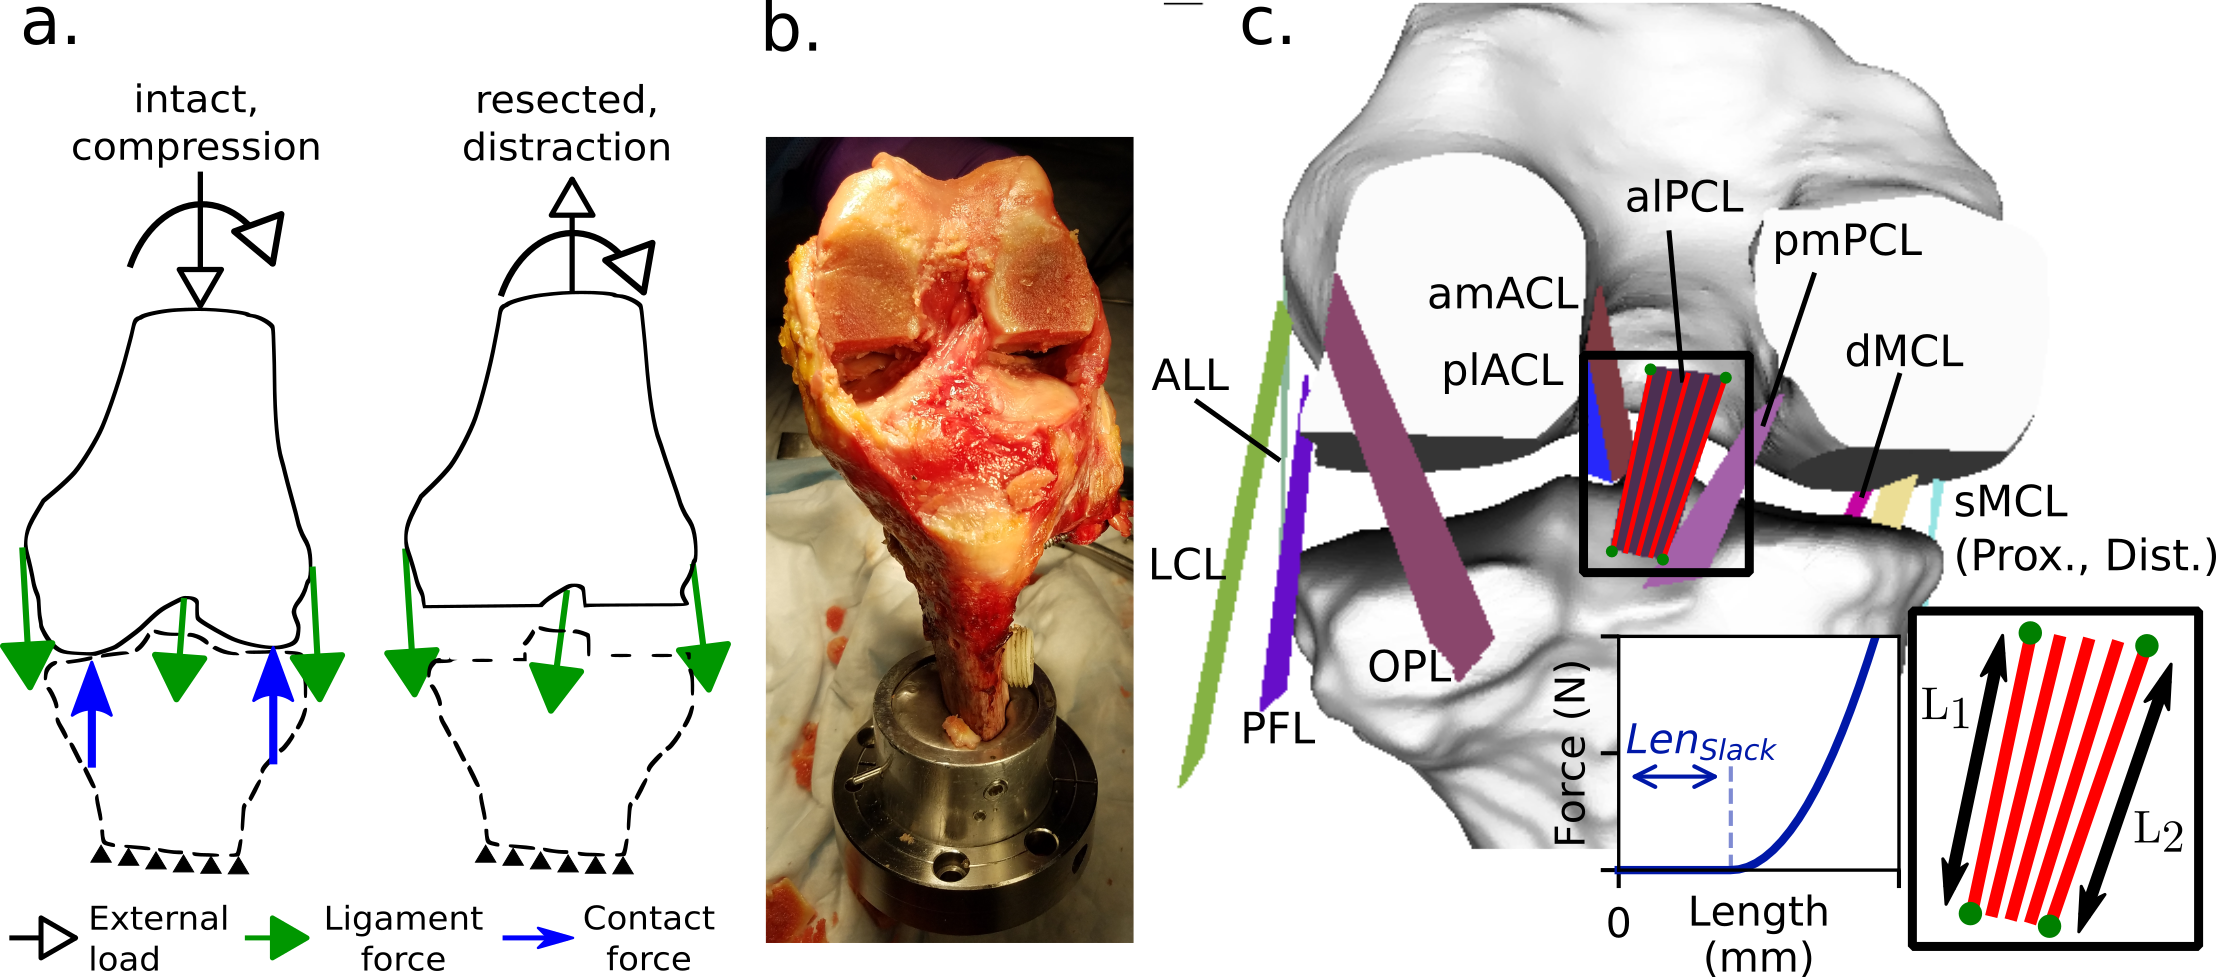
\includegraphics[width=0.85\linewidth]{../img/TwoColumnFig.png}
    \caption{(a) A similified representation of the joint forces during an intact laxity-style test compared to a distraction laxity-style test. (b) The specimen with resected femoral articulating surfaces. (c) The knee model with 11 ligament bundles represented. (inset) The non-linear spring model, and the definition of slack lenghth for a ligament with five fibers.}
    \label{fig:kneeModel}
\end{figure}

% ---------------------------------------------------
\section{Methods}
Specimen-specific geometry was defined using the specimen's MR images. The femur and the tibia were segmented, and 11 ligament bundles were defined using the MR images and literature descriptions (\autoref{fig:kneeModel}). The anterior and posterior cruciate ligaments were modeled as four bundles. These bundles were the anteromedial and posterolateral anterior cruciate ligament (amACL, plACL) \citep{duthon_anatomy_2006} and the anterolateral and posteromedial posterior cruciate ligament (alPCL, pmPCL) \citep{anderson_arthroscopically_2012}. The medial collateral ligament (MCL) was modeled as three bundles. Two of those bundles composed the proximal and distal superficial MCL (psMCL, dsMCL), and one bundle defined the deep MCL (dMCL)  \citep{laprade_anatomy_2007-1}. Additional ligament bundles included the lateral collateral ligament (LCL), the popliteofibular ligament (PFL) \citep{laprade_posterolateral_2003}, the anterolateral ligament (ALL) \citep{claes_anatomy_2013}, and the oblique popliteal ligament (OPL) \citep{laprade_anatomy_2007,hedderwick_oblique_2017}. 

The ligament bundles were defined by manually placing two points at the margins of femoral and tibial insertion sites (four points total). Each bundle consisted of 25 fibers, where two fibers connect the points that define the insertion area, and the remaining 23 fibers are evenly mapped between the margins. Each ligament fiber was modeled as a nonlinear spring (\cite{blankevoort_validation_1996}). Uniform stiffness was applied across each ligament, where the fiber stiffnesses summed to the ligament's equivalent stiffness (\autoref{tab:equivalentStiffness}).

\begin{table}
    \caption{The equivalent stiffness (N$/\epsilon$) of each ligament bundle with units of force per unit strain.}
    \label{tab:equivalentStiffness}
    \begin{tabular}{ r c p{9em}} \hline
        \textbf{Ligament} & \textbf{Stiffness} & \textbf{Reference} \\ \hline
        amACL & 2120 & \cite{amiri_mechanics_2007}, \cite{kia_multibody_2016} \\
        plACL & 2880 & \cite{amiri_mechanics_2007}, \cite{kia_multibody_2016} \\
        alPCL & 5625 & \cite{amiri_mechanics_2007}, \cite{kia_multibody_2016} \\
        pmPCL & 3375 & \cite{amiri_mechanics_2007}, \cite{kia_multibody_2016} \\
        psMCL & 1375 & \cite{amiri_mechanics_2007} \\
        dsMCL & 1375 & \cite{amiri_mechanics_2007} \\
        dMCL & 1000 & \cite{amiri_mechanics_2007} \\
        LCL & 2000 & \cite{amiri_mechanics_2007} \\
        ALL & 750 & \cite{ewing_estimating_2015} \\
        PFL & 1000 & \cite{ewing_estimating_2015} \\
        OPL & 1000 & \cite{ewing_estimating_2015} \\
        \hline
    \end{tabular}
\end{table}

Experimental kinetics were applied to the forward kinematics model, and the length of each ligament fiber was used to calculate the magnitude of force carried by each fiber. The line of action was defined using each fiber's femoral and tibial insertion point. Based on visualization of the kinematics, some ligaments simulated wrapping around either the femur, or a cylinder that approximated the tibia's surface. Tibial reaction forces were calculated by summing the force carried by each ligament fiber along its line of action \citep{mommersteeg_characterization_1996}, and when applicable, the wrapping reaction forces. Tibial reaction moments were calculated with tibial insertion points, wrapping points, and each fiber's force magnitude and line of action.

Ligament slack lengths were estimated using a constrained sequential quadratic programming algorithm. To simulate nonhomogeneous prestrain, two values were used to define ligament slack length for every fiber in a ligament bundle. The length of the two fibers at the margins of the insertion site was defined, and linear interpolation was used to define the slack length for the remaining fibers (\autoref{fig:kneeModel}). The optimization minimized the residual between the model and experimentally measured tibial reaction forces for the anterior-posterior drawer and fixed varus-valgus distraction tests at 0\textsuperscript{o}, 30\textsuperscript{o}, 60\textsuperscript{o}, 90\textsuperscript{o} flexion (\autoref{eq:Optimization}).

\begin{equation}
    \begin{aligned}
    & \underset{\bm{x}}{\text{minimize}}
    & & f(\bm{x}) = \sum_{j=1}^{72}\sum_{j=1}^6 \big[w_j(M_{ij}(\bm{x}) - E_{ij})\big]^2 \\
    & \text{subject to} \\
    & & h(x_m) &\geq 0.1, \; m = 1, \ldots, 22
    \end{aligned}
    \label{eq:Optimization}
\end{equation}

Where $i$ is number of the step in the loading cycle, and $j$ is the force degree of freedom. The weighting factor ($w$) applied a weight of 1 to the forces, and a weight of 20 to the moments. Three experimental tests were excluded from the optimization to evaluate the inverse modeling scheme's performance. 

\section{Results and Discussion}
For the tests that were included in the optimization (anterior-posterior drawer and varus-valgus), the RMS error of the joint kinetics across all flexion angles was 5.8 N, 22.5 N and 17.1 N for the medial, anterior, and superior loads respectively, and 0.80 Nm, 0.60 Nm, and 0.33 Nm for the extension, valgus, and internal rotation moments respectively (\autoref{fig:optimizationAPResults}, \autoref{fig:optimizationVVResults}).

\begin{figure}
    \centering
    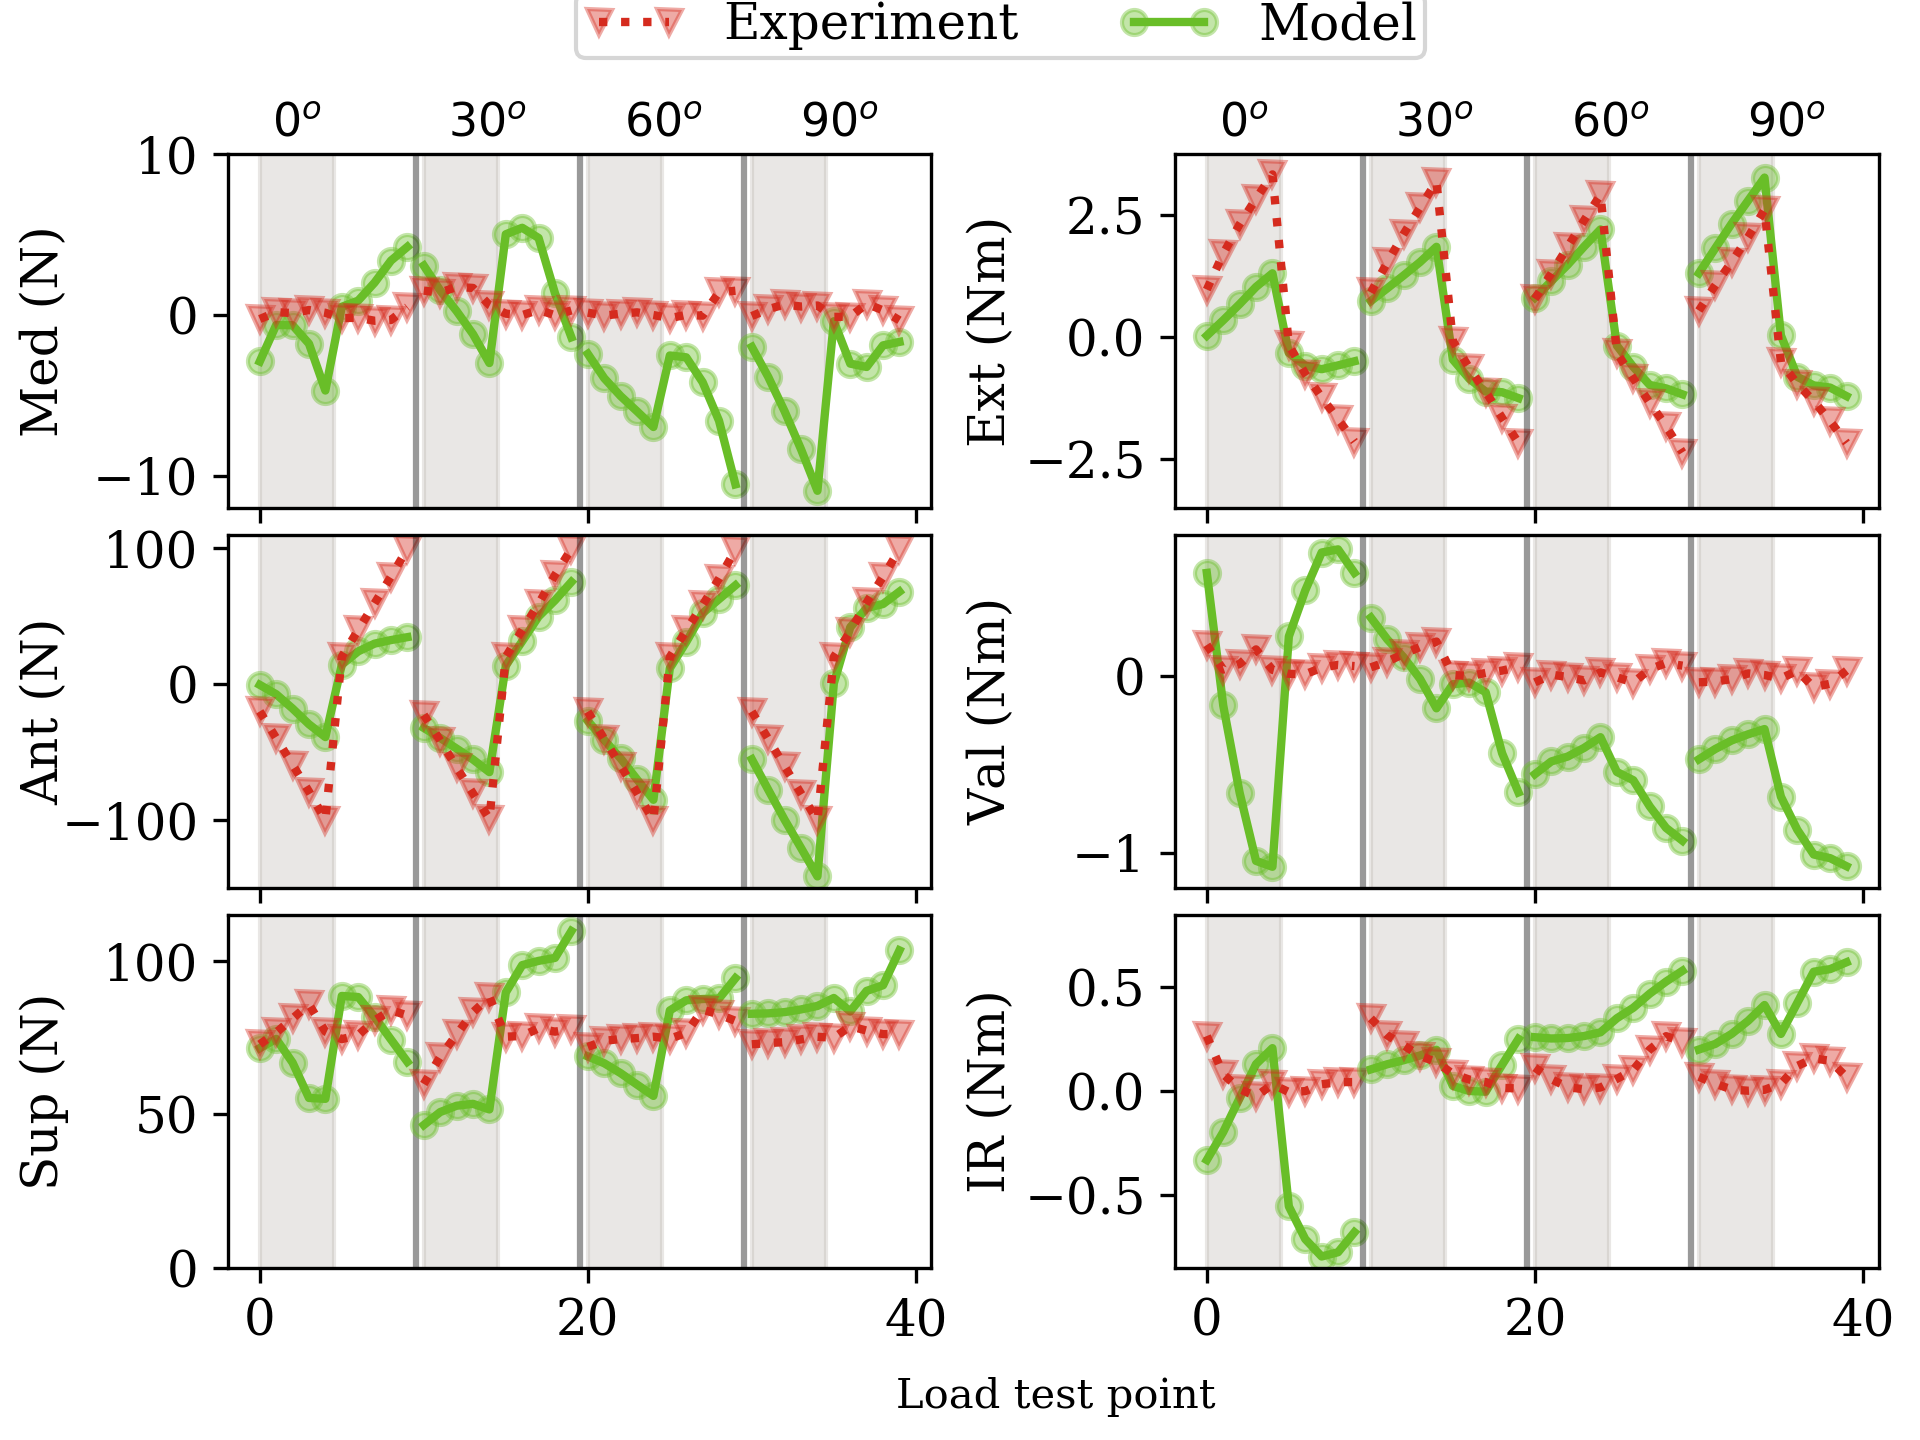
\includegraphics[width=0.80\linewidth]{../img/Spec1_AP_OptimizationResults_APVV_0_30_60_90.png}
    \caption{Tibial reaction forces and moments for the (grey) anterior and (white) posterior drawer tests for the experiment and calibrated model at 0\textsuperscript{o}, 30\textsuperscript{o}, 60\textsuperscript{o}, 90\textsuperscript{o} flexion. Med, Ant, Sup are the medial, anterior, and superior tibial reaction forces, respectively. Ext, Val, IR are the extension, valgus, and internal tibial rotation reaction moments, respectively.}
    \label{fig:optimizationAPResults}
\end{figure}

\begin{figure}
    \centering
    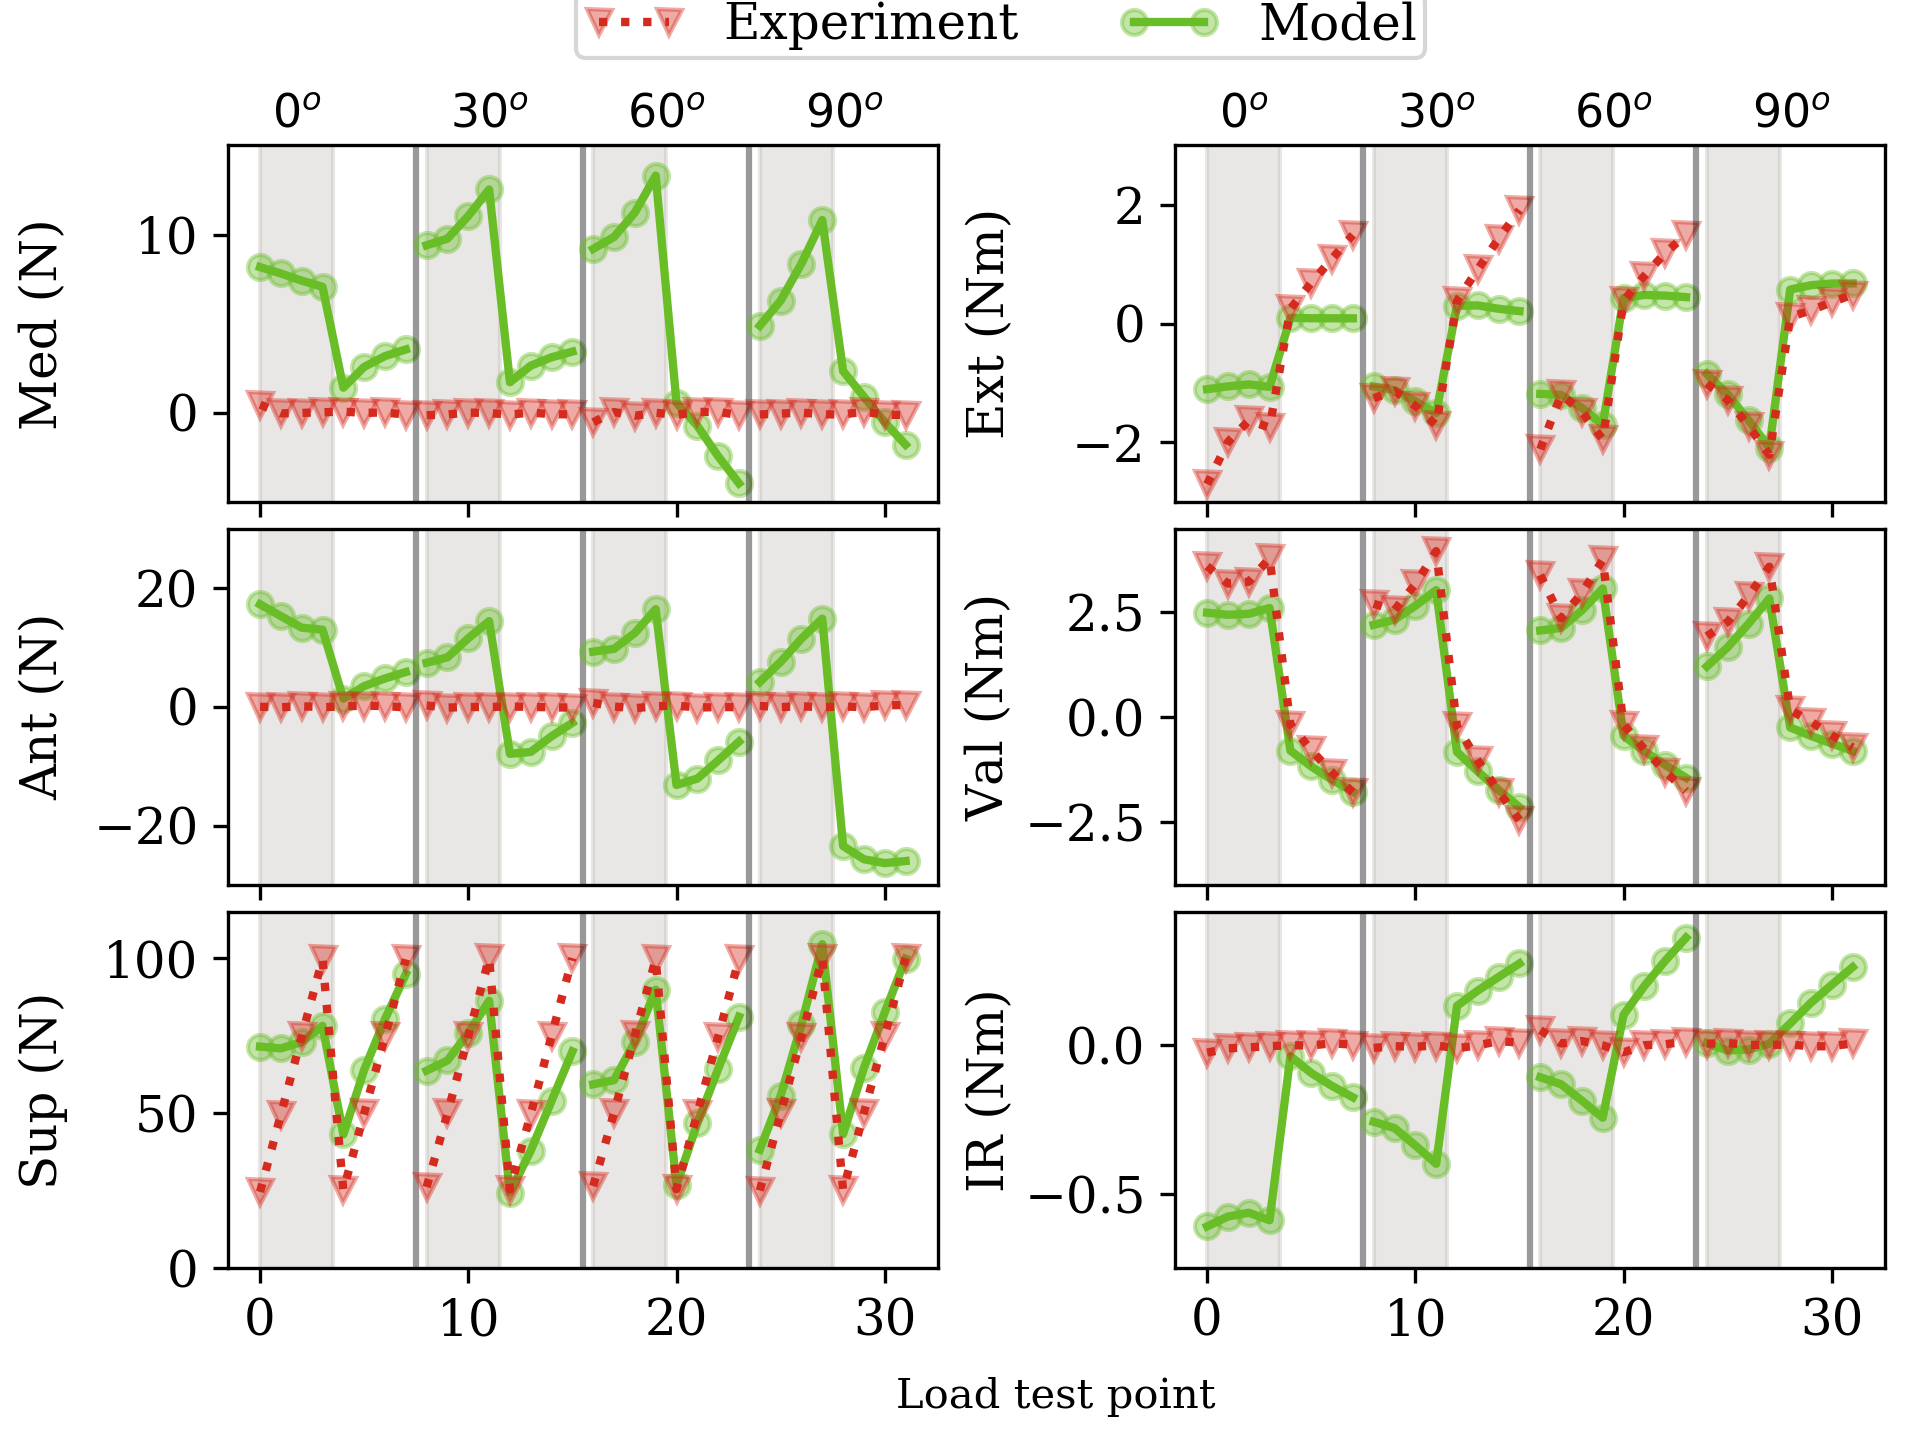
\includegraphics[width=0.80\linewidth]{../img/Spec1_VV_OptimizationResults_APVV_0_30_60_90.png}
    \caption{Tibial reaction forces and moments for the (grey) varus and (white) valgus tests for the experiment and calibrated model at 0\textsuperscript{o}, 30\textsuperscript{o}, 60\textsuperscript{o}, 90\textsuperscript{o} flexion. Med, Ant, Sup are the medial, anterior, and superior tibial reaction forces, respectively. Ext, Val, IR are the extension, valgus, and internal tibial rotation reaction moments, respectively.}
    \label{fig:optimizationVVResults}
\end{figure}

For the distraction test, which was not part of the optimization, the RMS error of the joint kinetics across all flexion angles was 2.5 N, 13.4 N and 14.2 N for the medial, anterior, and superior loads respectively, and 0.54 Nm, 0.36 Nm, and 0.31 Nm for the extension, valgus, and internal rotation moments respectively (\autoref{fig:resultsDistraction}).

\begin{figure}
    \centering
    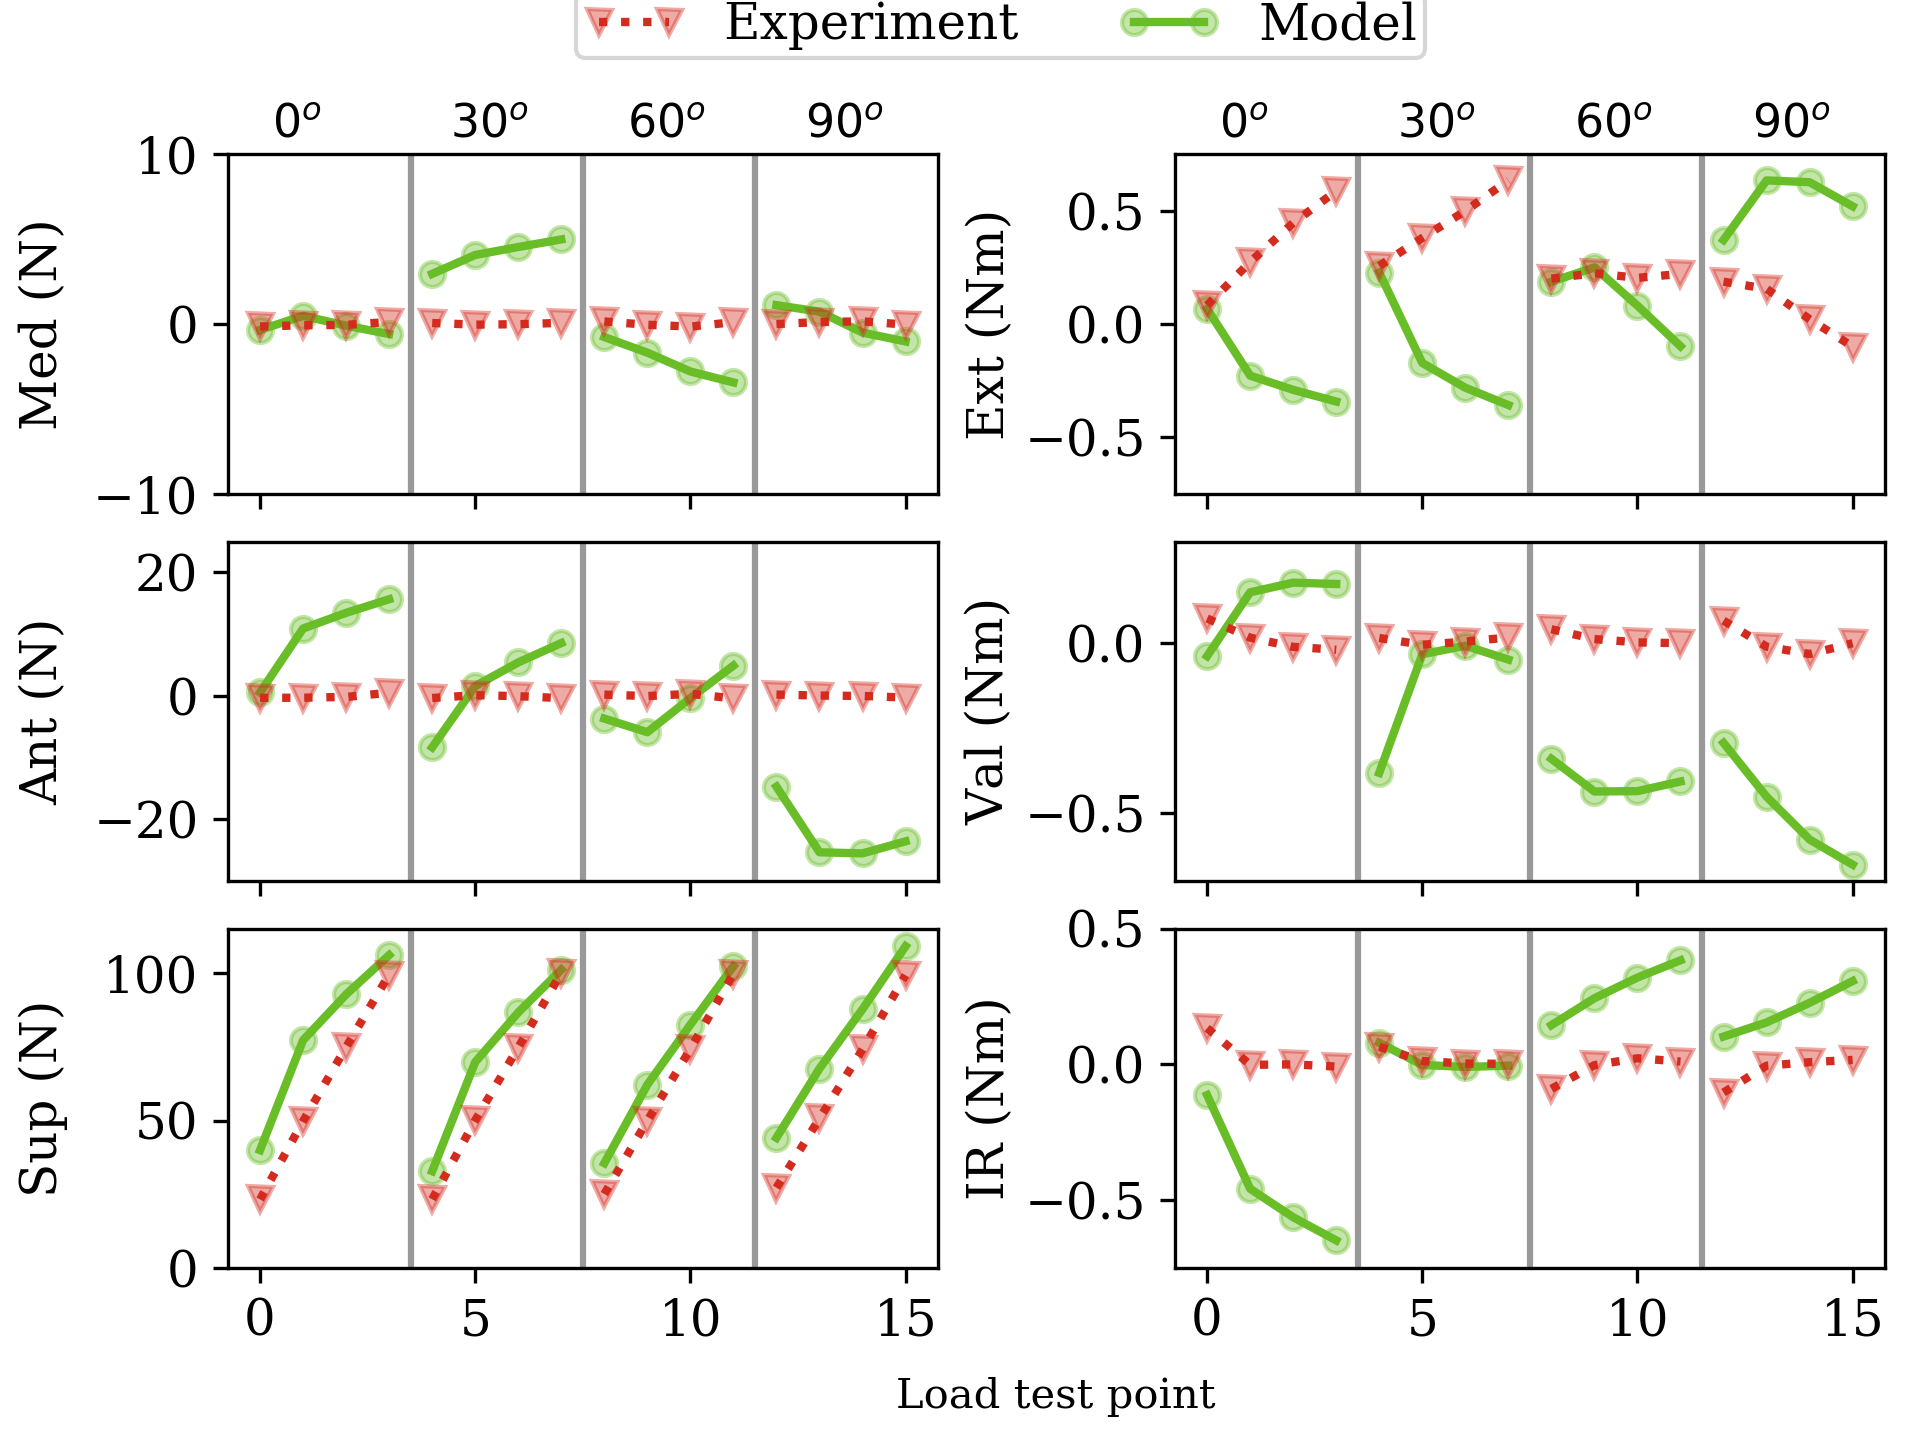
\includegraphics[width=0.80\linewidth]{../img/Spec1_Dist_OptimizationResults_APVV_0_30_60_90.png}
    \caption{Tibial reaction forces and moments for the calibrated model compared to the experimentally measured values for the distraction test. Results are shown for 0\textsuperscript{o}, 30\textsuperscript{o}, 60\textsuperscript{o}, 90\textsuperscript{o} flexion. This test was not included in the optimization. Med, Ant, Sup are the medial, anterior, and superior tibial reaction forces, respectively. Ext, Val, IR are the extension, valgus, and internal tibial rotation reaction moments, respectively.}
    \label{fig:resultsDistraction}
\end{figure}

For the kinetic plane and distraction tests, the highest errors in anterior force occurred at 90\textsuperscript{o} flexion, and the highest distraction force errors occurred at 0\textsuperscript{o} flexion (\autoref{tab:distResults}). The internal-external rotation model demonstrated the largest difference in distraction force (\autoref{tab:distResults}). For the internal-external rotation tests, the model performed better when the applied torque was lower. Across flexion angles, the RMS distraction force error was 13.5 N at $\pm$ 1 Nm internal rotation torque, and 46.2 N at $\pm$ 5 Nm internal rotation torque.

\begin{table}
    \caption{RMS errors between the experimental and calibrated model joint reaction forces (N) and moments (Nm) for the distraction, kinetic plane, and external-internal rotation tests. These tests were not part of the optimization.}
    \label{tab:distResults}
    \setlength{\tabcolsep}{10pt}
    \begin{tabular}{ l l c c c c c c } \hline
        \textbf{Flexion} & \textbf{Test} & $F_{med}$ & $F_{ant}$ & $F_{sup}$ & $M_{ext}$ & $M_{val}$ & $M_{ir}$\\ \hline
        \multirow{4}{*}{0\textsuperscript{o}}& K. Pl. & 9.87 & 19.29 & 10.47 & 1.06 & 0.18 & 0.66\\
        & Dist. & 0.46 & 11.64 & 18.68 & 0.64 & 0.16 & 0.50\\
        & ER  & 2.73 & 11.94 & 13.41 & 1.00 & 0.21 & 2.72\\
        & IR  & 3.67 & 20.99 & 28.32 & 2.00 & 0.93 & 3.32\\
        \hline 
        \multirow{4}{*}{30\textsuperscript{o}}& K. Pl. & 11.84 & 11.07 & 9.85 & 1.01 & 0.17 & 0.07\\
        & Dist. & 4.19 & 6.63 & 12.48 & 0.69 & 0.20 & 0.01\\
        & ER  & 3.60 & 9.03 & 32.09 & 0.94 & 0.99 & 2.86\\
        & IR  & 6.07 & 36.09 & 45.38 & 1.25 & 0.34 & 3.24\\
        \hline 
        \multirow{4}{*}{60\textsuperscript{o}}& K. Pl. & 8.65 & 6.45 & 9.09 & 0.42 & 0.44 & 0.37\\
        & Dist. & 2.41 & 4.42 & 9.13 & 0.17 & 0.42 & 0.29\\
        & ER  & 0.81 & 9.70 & 53.11 & 0.61 & 0.60 & 3.02\\
        & IR  & 2.30 & 13.58 & 59.35 & 0.82 & 0.29 & 3.24\\
        \hline 
        \multirow{4}{*}{90\textsuperscript{o}}& K. Pl. & 7.58 & 25.15 & 7.99 & 0.72 & 0.65 & 0.30\\
        & Dist. & 0.87 & 22.71 & 14.62 & 0.50 & 0.51 & 0.22\\
        & ER  & 5.58 & 6.43 & 43.39 & 0.93 & 0.45 & 2.72\\
        & IR  & 3.66 & 18.70 & 33.68 & 0.33 & 0.36 & 2.71\\
        \hline 
        \end{tabular}
    \begin{tablenotes}
        \small
        \item K. Pl.: kinetic plane test, Dist.: distraction test, ER.: external tibial rotation test, IR.: internal tibial rotation test.
        \item $F_{med}$, $F_{ant}$, $F_{sup}$: medial, anterior and superior tibial reaction forces, respectively.
        \item $M_{ext}$, $M_{val}$, $M_{ir}$: extension, valgus, and internal tibial rotation tibial reaction moments, respectively.
    \end{tablenotes}
\end{table}